\documentclass[Bachelorarbeit.tex]{subfiles}
\begin{document}

\graphicspath{{./figures/results/}}	%specifying the folder for the figures

\chapter{Results}
\label{ch:results}

In this chapter the results of the experiments are given. Each topology-type introduced in appendix \ref{app:topologies} "Topologies" was simulated where in this chapter only Fully-Connected and Ascending-Connected topologies are handled as the Ascending-Connected topology - both with and without importance sampling - is the most minimal network which satisfies the requirements for the hypothesis. The results for the other topologies can be found in appendix \ref{app:results} "Results for Hub-Based, Scale-Free and Small-World Topologies".

Note: The numbers in tables resemble always a median-value with the standard-deviation given in parentheses.

\section{Validating simulation results}
As  a point-of-reference and as an experimental proof for the correctness of the implementation of the thesis-software the results of a validation against both the theoretical equilibrium and the equilibrium found in \cite{Breuer2015} are given. Because equilibrium differs across the number of agents and the type of bond traded to be comparable the same amount of agents and the same bond-type has to be used in the experiments which is 1000 Agents and a bond with face-value of 0.5 because \cite{Breuer2015} report their equilibria only for a count of 1000 agents and bonds with face-value between 0.1 to 0.5.

\subsection{References}

\begin{table}[H]
	\centering
	\caption{Theoretical equilibrium for 1,000 agents and 0.5 bond}
	\begin{tabular} { l c r }
		\hline
		Asset-Price p & 0.715 \\
		Bond-Price q & 0.374 \\
		Marginal agent i1 & 0.583 \\
		Marginal agent i2 & 0.802 \\
		\hline
	\end{tabular}
	\label{tab:equilibrium_THEORY_1000}
\end{table}

\begin{table}[H]
	\centering
	\caption{Equilibrium in \cite{Breuer2015} for 1,000 agents and 0.5 bond}
	\begin{tabular} { l c r }
		\hline
		Asset-Price p & 0.716 \\
		Bond-Price q & 0.375 \\
		Marginal agent i1 & 0.583 \\
		Marginal agent i2 & 0.801 \\
		\hline
		Pessimist Wealth & 1.716 \\
		Medianist Wealth & 4.578 \\
		Optimist Wealth & 5.032 \\
		\hline
	\end{tabular}
	\label{tab:equilibrium_BREUER_1000}
\end{table}

\subsection{Thesis results}

\begin{figure}[H]
	\centering
  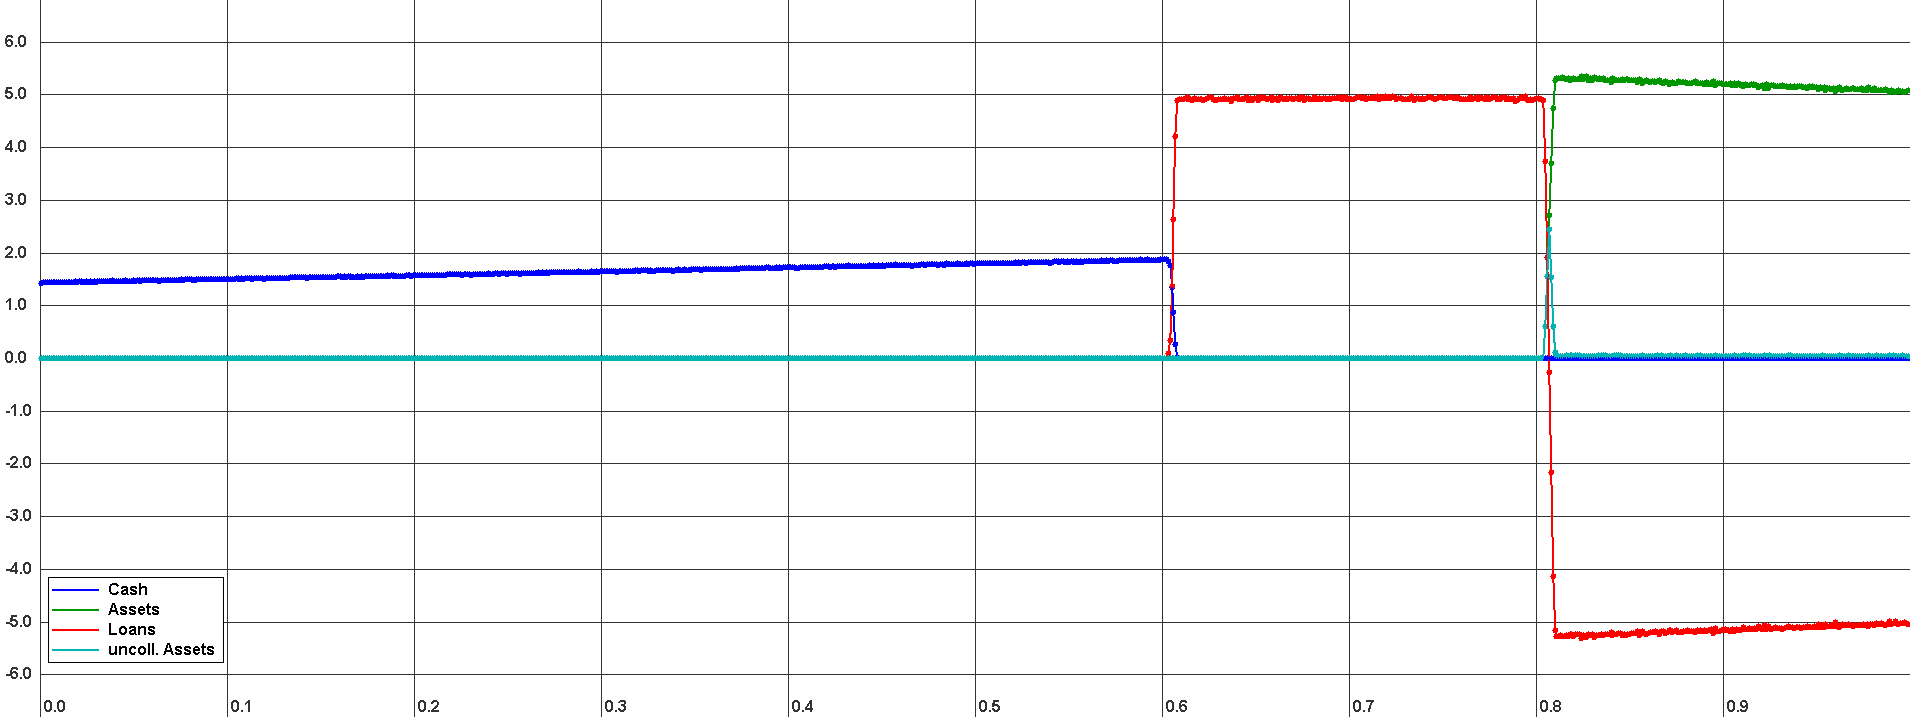
\includegraphics[width=1.0\textwidth, angle=0]{FULLYCONNECTED_1000_NOCOLLATERALMARKET_REPL.png}
	\caption{Wealth-Distribution of thesis-implementation of Fully-Connected topology for 1,000 agents and 0.5 bond}
	\label{fig:wealth_FULLYCONNECTED_1000_NOCOLLATERALMARKET_REPL}
\end{figure}

\begin{table}[H]
	\centering
	\caption{Equilibrium of thesis-implementation for 1,000 agents and 0.5 bond}
	\begin{tabular} { l c r }
		\hline
		Asset-Price p & 0.700 (0.005) \\
		Bond-Price q & 0.389 (0.002) \\
		Marginal agent i1 & 0.616 (0.004) \\
		Marginal agent i2 & 0.805 (0.001) \\
		\hline
		Pessimist Wealth & 1.582 (0.01) \\
		Medianist Wealth & 4.578 (0.031) \\
		Optimist Wealth & 5.105 (0.025) \\
		\hline
	\end{tabular}
	\label{tab:equilibrium_THESIS_1000_50_REPL}
\end{table}

\begin{table}[H]
	\caption{Difference of Fully-Connected topology equilibrium as given in table \ref{tab:equilibrium_THESIS_1000_50_REPL} to theoretical equilibrium as given in table \ref{tab:equilibrium_THEORY_1000}}
	\centering
	\begin{tabular} { l c c c r }
		& Result & Reference & difference to Reference \\
		\hline
		Asset-Price p & 0.700 & 0.715 & -2.1\% \\
		Bond-Price q & 0.389 & 0.374 & +4.0\% \\
		Marginal agent i1 & 0.616  & 0.583 & +5.6\% \\
		Marginal agent i2 & 0.805 & 0.802 & +0.4\% \\
		\hline
	\end{tabular}
\end{table} 

\begin{table}[H]
	\caption{Difference of Fully-Connected topology wealth-equilibrium as given in table \ref{tab:equilibrium_THESIS_1000_50_REPL} to wealth-equilibrium as given in \cite{Breuer2015} from table \ref{tab:equilibrium_BREUER_1000}}
	\centering
	\begin{tabular} { l c c c r }
		& Result & Reference & difference to Reference \\
		\hline
		Pessimist Wealth  & 1.582 & 1.716 & -7.8\% \\
		Medianist Wealth & 4.578 & 4.578 & 0.0\% \\
		Optimist Wealth & 5.105 & 5.032 & +1.5\% \\
		\hline
	\end{tabular}
\end{table} 

Although marginal agent i1 and bond-price q are quite different than from theoretical equilibrium and the pessimists wealth is 7.8\% less than given in \cite{Breuer2015} these results are accepted as reaching the equilibrium. The differences emerge from the reasons that the thesis-simulation runs were terminated earlier than in \cite{Breuer2015} which results in the i1 and i2 edges to be not as sharp as reported in \cite{Breuer2015}. It would be necessary to run the simulation an order of magnitude longer as the matching probabilities are reduced rapidly when only direct neighbours are able to trade any more within a network of 1000 agents. See section \ref{sec:implementation_performanceImprovement} "Performance improvement" for details on matching-probabilities.

\subsection{Performance Measurements}
As noted in section \ref{sec:implementation_sweepingAndMatching} "Sweeping and Matching" a matching-round performs up to 500 offering-rounds where during one round all agents make an offer to find a match. If a match occurs during one offering-round the current matching-round is terminated and marked as successful. If no match occurs during all 500 offering-rounds the current matching-round is terminated too but marked as failed. Thus the following terminology is defined:

\paragraph{Successful matching-round} a match occurred within maximal 500 offering-rounds where in each offering-round all agents make an offer.
\paragraph{Failed matching-round} no match occurred within 500 offering-rounds where in each offering-round all agents make an offer.

\begin{table}[H]
	\centering
	\caption{Performance of thesis-implementation with 1000 agents and 0.5 bond}
	\begin{tabular} { l c r }
		\hline
		Successful matching-rounds & 19,300.04 (101.68) \\
		Failed matching-rounds & 10,306.78 (2914.11) \\
		Total matching-rounds & 29,606.82 (2938.82) \\
		\hline
		Ratio successful/total & 0.65 \\
		Ratio failed/total & 0.35 \\
		\hline
	\end{tabular}
\end{table}


\section{Experiments configuration}
In the following experiments 100 agents were used, all markets (Asset/Cash, Bond/Cash, Asset/Bond) were enabled, a bond with face-value of 0.5 was selected and the number of replications run was 50. A replication was terminated after 1000 failed matching-rounds in a row. Note that if trading is not possible any more before 1000 failed matching-rounds have been reached in a row, the simulation is terminated too and thus it is possible that it halts earlier as can be seen for the Ascending-Connected Importance Sampling topology.

\bigskip 

\cite{Breuer2015} showed that equilibrium can be reached already with 30 agents so this was the minimum number of agents to start with but for a smoother visual result 100 were chosen. Also one simulation-run takes not very much time with 100 as compared to the 1000 agents thus it is a very good match between visual accurateness and processing-power requirements.

\medskip

The 0.5 bond was selected because it is a risky one which is important as with risk-less loans which have a face-value less than 0.2 the results are indifferent and not unique and won't show the characteristic distribution of equilibrium.

\medskip

As already described in section \ref{sec:implementation_sweepingAndMatching} "Sweeping and Matching" the whole simulation-process is a random-process with an equilibrium different for each topology as the fixed-point solution thus one needs replications to reduce noise. The number of 50 replications was chosen because it is a good match between processing-power requirements and overall reduction of noise. Thus increasing the number e.g. to 100 or 200 would not result in much better results - both visual and numerical - but would need much longer to run. All facts can already be seen and derived when using 50 replications thus for all figures 50 replications were used unless stated otherwise e.g. a single run.

\begin{table}[H]
	\centering
	\caption{Configuration for all experiments}
	\begin{tabular} { l c r }
		\hline
		Agent-Count & 100 \\
		Bond-Type & 0.5 \\
		Replication-Count & 50 \\
		Matching-Round & max. 500 offering-rounds \\
		Terminate after & 1000 failed successive matching-rounds \\
		\hline
	\end{tabular}
\end{table}

\begin{table}[H]
	\centering
	\caption{Theoretical Equilibrium for 100 agents and 0.5 bond}
	\begin{tabular} { l c r }
		\hline
		Asset-Price p & 0.717 \\
		Bond-Price q & 0.375 \\
		Marginal agent i1 & 0.584 \\
		Marginal agent i2 & 0.802 \\
		\hline
	\end{tabular}
	\label{tab:theoretical_equilibrium_100Agents_05Bond}
\end{table}

\section{Fully-Connected}
This topology serves as the major point-of-reference for the other experiments as it reaches the theoretical equilibrium for 1000 agents as demonstrated and explained.

\begin{figure}[H]
	\centering
  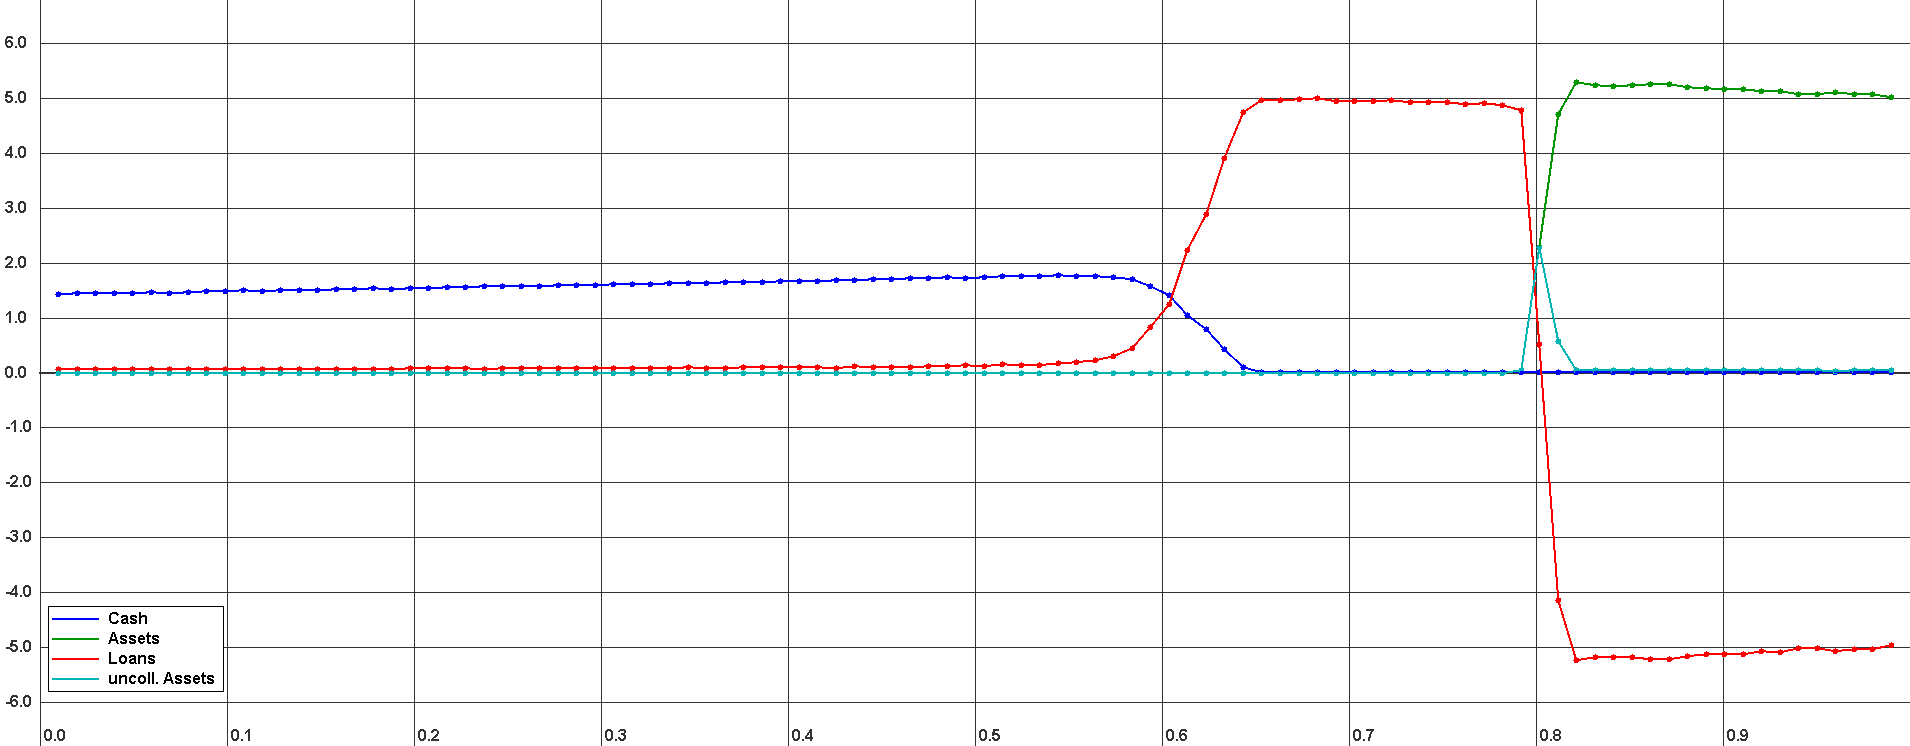
\includegraphics[width=1.0\textwidth, angle=0]{FULLYCONNECTED_100_NOCOLLATERALMARKET_REPL.png}
	\caption{Wealth-distribution of Fully-Connected topology}
	\label{fig:wealth_FULLYCONNECTED_100_NOCOLLATERALMARKET_REPL}
\end{figure}

\begin{table}[H]
	\caption{Equilibrium of Fully-Connected topology}
	\centering
	\begin{tabular} { l c r }
		\hline
		Asset-Price p & 0.689 (0.01) \\
		Bond-Price q & 0.384 (0.004) \\
		Marginal agent i1 & 0.603 (0.007) \\
		Marginal agent i2 & 0.803 (0.003) \\
		\hline
		Pessimist Wealth & 1.597 (0.015) \\
		Medianist Wealth & 4.565 (0.113) \\
		Optimist Wealth & 5.021 (0.064) \\
		\hline
	\end{tabular}
	\label{tab:fullyconnected_equilibrium_100Agents_05Bond}
\end{table} 

\begin{table}[H]
	\caption{Difference to theoretical equilibrium}
	\centering
	\begin{tabular} { l c c c r }
		& Result & Reference & difference to Reference \\
		\hline
		Asset-Price p & 0.689 & 0.717 & -3.9\% \\
		Bond-Price q & 0.384 & 0.375 & +2.4\% \\
		Marginal agent i1 & 0.603  & 0.584 & +3.2\% \\
		Marginal agent i2 & 0.803 & 0.802 & +0.1\% \\
		\hline
	\end{tabular}
\end{table}

\begin{table}[H]
	\caption{Performance of Fully-Connected topology}
	\centering
	\begin{tabular} { l c r }
		\hline
		Successful matching-rounds & 1916.14 (31.42) \\
		Failed matching-rounds & 4448.66 (1668.93) \\
		Total matching-rounds & 6364.8 (1679.21) \\
		\hline
		Ratio successful/total & 0.3 \\
		Ratio failed/total & 0.7 \\
		\hline
	\end{tabular}
\end{table}

\section{Ascending-Connected topology} 

\begin{figure}[H]
	\centering
  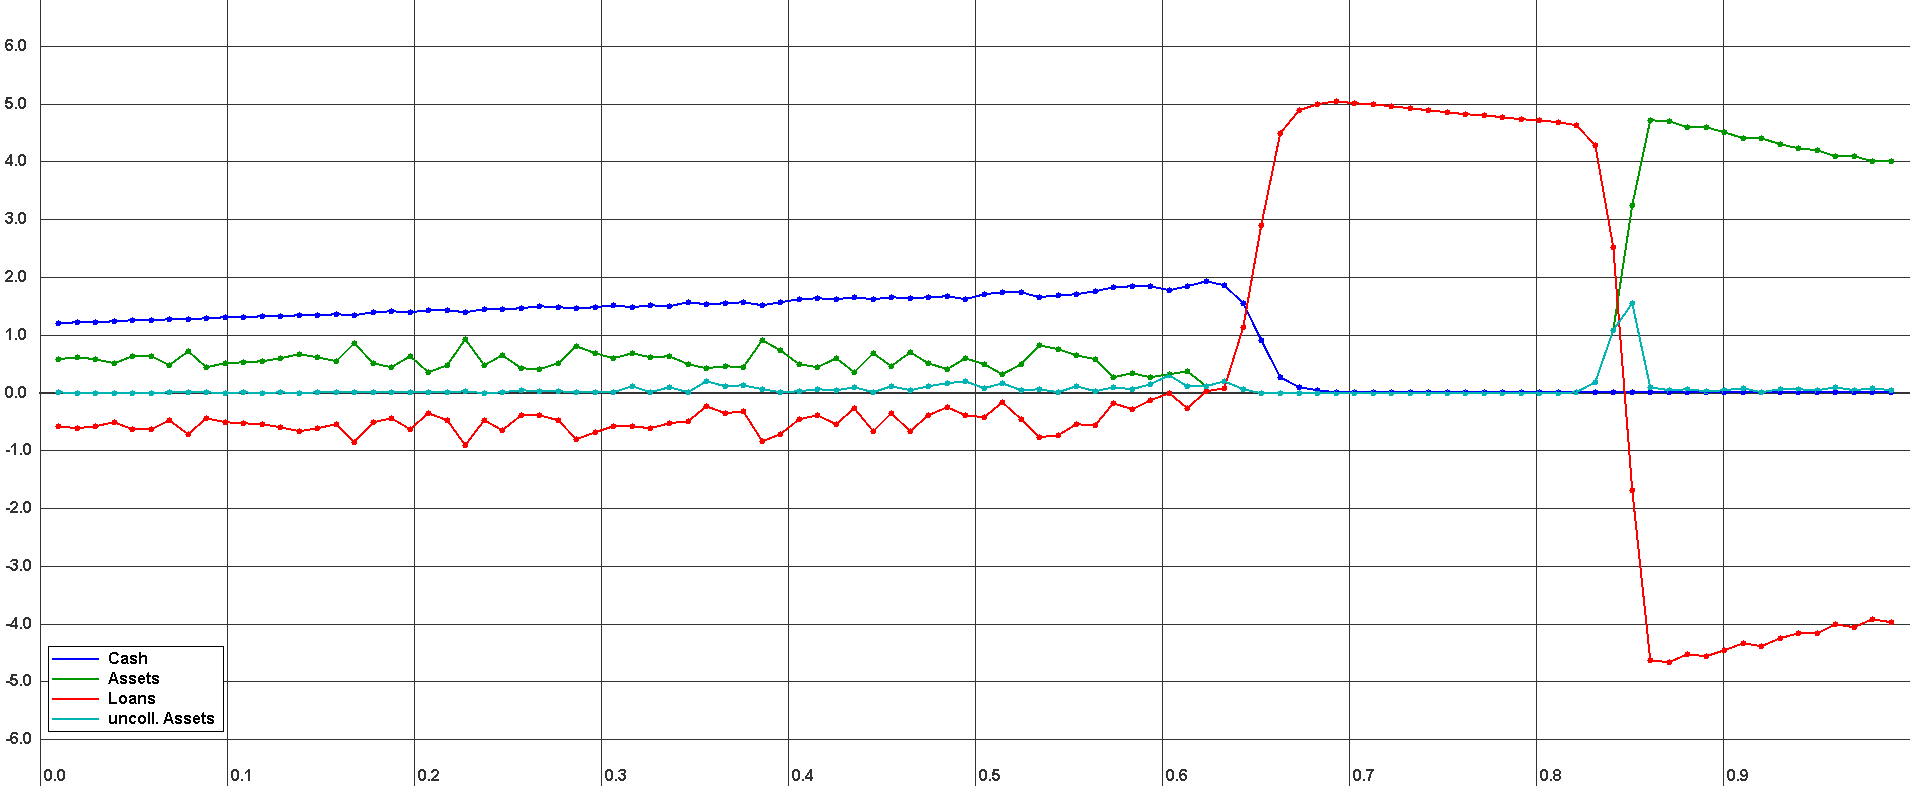
\includegraphics[width=1.0\textwidth, angle=0]{ASCENDINGCONNECTED_100_NOCOLLATERALMARKET_REPL.png}
	\caption{Wealth-distribution of Ascending-Connected topology}
	\label{fig:wealth_ASCENDINGCONNECTED_100_NOCOLLATERALMARKET_REPL}
\end{figure}

\begin{table}[H]
	\caption{Equilibrium of Ascending-Connected topology}
	\centering
	\begin{tabular} { l c r }
		\hline
		Asset-Price p & 0.711 (0.016) \\
		Bond-Price q & 0.391 (0.005) \\
		Marginal agent i1 & 0.646 (0.012) \\
		Marginal agent i2 & 0.850 (0.008) \\
		\hline
		Pessimist Wealth & 1.166 (0.072) \\
		Medianist Wealth & 1.869 (0.243) \\
		Optimist Wealth & 4.307 (0.07) \\
		\hline
	\end{tabular}
	\label{tab:ascendingconnected_equilibrium_100Agents_05Bond}
\end{table} 

\begin{table}[H]
	\caption{Performance of Ascending-Connected topology}
	\centering
	\begin{tabular} { l c r }
		\hline
		Successful matching-rounds & 36,940.96 (1948.69) \\
		Failed matching-rounds & 1176.08 (98.01) \\
		Total matching-rounds & 38,117.04 (1934.06) \\
		\hline
		Ratio successful/total & 0.97 \\
		Ratio failed/total & 0.03 \\
		\hline
	\end{tabular}
\end{table}

\begin{table}[H]
	\caption{Difference to theoretical equilibrium}
	\centering
	\begin{tabular} { l c c c r }
		& Result & Reference & difference to Reference \\
		\hline
		Asset-Price p & 0.711 & 0.717 & -0.8\% \\
		Bond-Price q & 0.391 & 0.375 & +4.2\% \\
		Marginal agent i1 & 0.646  & 0.584 & +10.6\% \\
		Marginal agent i2 & 0.850 & 0.802 & +6.0\% \\
		\hline
	\end{tabular}
\end{table}

\begin{table}[H]
	\caption{Difference to Fully-Connected topology equilibrium}
	\centering
	\begin{tabular} { l c c c r }
		& Result & Reference & difference to Reference \\
		\hline
		Asset-Price p & 0.711 (0.016) & 0.689 (0.01) & +3.2\% (+60\%) \\
		Bond-Price q & 0.391 (0.005) & 0.384 (0.004) & +1.8\% (+25\%) \\
		Marginal agent i1 & 0.646 (0.012) & 0.603 (0.007) & +6.9\% (+71\%) \\
		Marginal agent i2 & 0.850 (0.008) & 0.803 (0.003) & +6.0\% (+166\%) \\
		\hline
		Pessimist Wealth & 1.166 (0.072) & 1.597 (0.015) & -27.0\% (+380\%) \\
		Medianist Wealth & 1.869 (0.243) & 4.565 (0.113) & -59\% (+115\%) \\
		Optimist Wealth & 4.307 (0.070) & 5.021 (0.064) & -14.2\% (+9.3\%) \\
		\hline
	\end{tabular}
\end{table}

\subsection{Ascending-Connected Importance Sampling}
\begin{figure}[H]
	\centering
  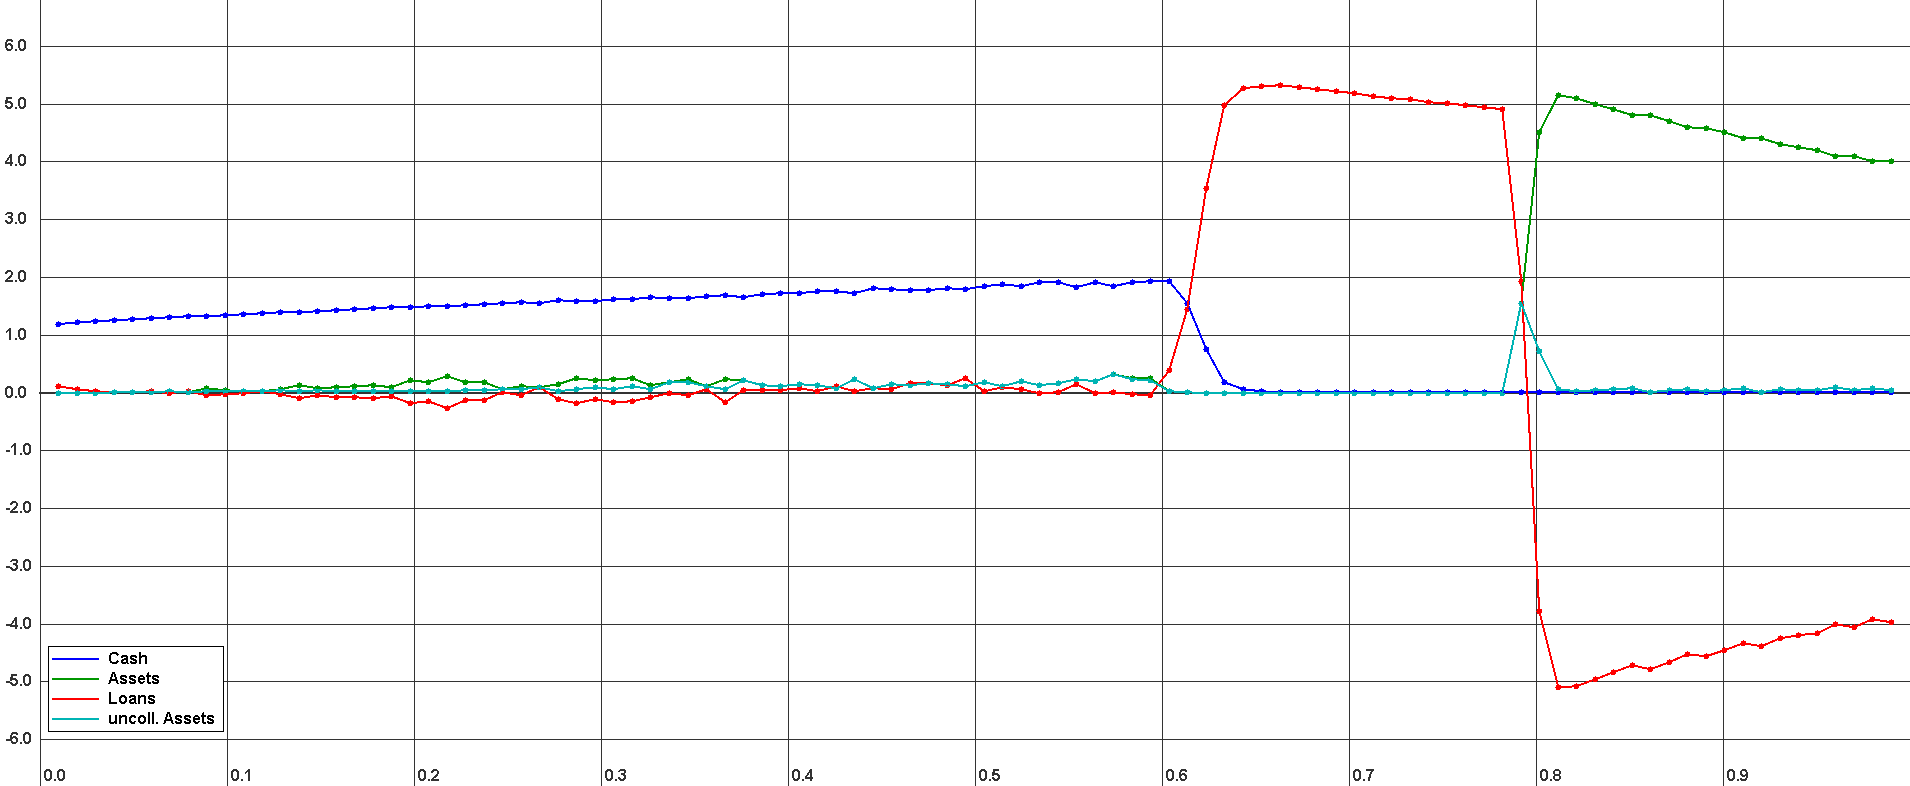
\includegraphics[width=1.0\textwidth, angle=0]{ASCENDINGCONNECTED_IS_100_NOCOLLATERALMARKET_REPL.png}
	\caption{Wealth-distribution of Ascending-Connected Importance Sampling topology}
	\label{fig:wealth_ASCENDINGCONNECTED_IS_100_NOCOLLATERALMARKET_REPL}
\end{figure}

\begin{table}[H]
	\caption{Equilibrium of Ascending-Connected Importance Sampling topology}
	\centering
	\begin{tabular} { l c r }
		\hline
		Asset-Price p & 0.691 (0.009) \\
		Bond-Price q & 0.383 (0.004) \\
		Marginal agent i1 & 0.614 (0.009) \\
		Marginal agent i2 & 0.799 (0.006) \\
		\hline
		Pessimist Wealth & 1.497 (0.072) \\
		Medianist Wealth & 3.934 (0.505) \\
		Optimist Wealth & 4.519 (0.051) \\
		\hline
	\end{tabular}
\end{table} 

\begin{table}[H]
	\caption{Performance of Ascending-Connected Importance Sampling topology}
	\centering
	\begin{tabular} { l c r }
		\hline
		Successful matching-rounds & 49,881.6 (1733.33) \\
		Failed matching-rounds & 1.0 (0.00) \\
		Total matching-rounds & 49,882.6 (1733.33) \\
		\hline
		Ratio successful/total & 0.9999 \\
		Ratio failed/total & 0.0001 \\
		\hline
	\end{tabular}
\end{table}

Note that in this case the matching-probabilities are such that upon the first failed matching-round the equilibrium is reached as no agent can trade with each other any more which results in just on single failed matching-round.

\begin{table}[H]
	\caption{Difference to theoretical equilibrium}
	\centering
	\begin{tabular} { l c c c r }
		& Result & Reference & difference to Reference \\
		\hline
		Asset-Price p & 0.691 & 0.717 & -3.6\% \\
		Bond-Price q & 0.383 & 0.375 & +2.1\% \\
		Marginal agent i1 & 0.614 & 0.584 & 5.1\% \\
		Marginal agent i2 & 0.799 & 0.802 & -0.4\% \\
		\hline
	\end{tabular}
\end{table}

\begin{table}[H]
	\caption{Difference to Fully-Connected topology equilibrium}
	\centering
	\begin{tabular} { l c c c r }
		& Result & Reference & difference to Reference \\
		\hline
		Asset-Price p & 0.691 (0.009) & 0.689 (0.01) & +0.3\% (-10\%) \\
		Bond-Price q & 0.383 (0.004) & 0.384 (0.004) & -0.3\% (0.0\%) \\
		Marginal agent i1 & 0.614 (0.009) & 0.603 (0.007) & +1.8\% (28.6\%) \\
		Marginal agent i2 & 0.799 (0.006) & 0.803 (0.003) & -0.5\% (+100\%) \\
		\hline
		Pessimist Wealth & 1.497 (0.072) & 1.597 (0.015) & -6.2\% (+380\%) \\
		Medianist Wealth & 3.934 (0.505) & 4.565 (0.113) & -13.8\% (+346\%) \\
		Optimist Wealth & 4.519 (0.051) & 5.021 (0.064) & -10\% (-20.3\%) \\
		\hline
	\end{tabular}
\end{table}
\end{document}
